% GNUPLOT: LaTeX picture with Postscript
\begingroup
  \makeatletter
  \providecommand\color[2][]{%
    \GenericError{(gnuplot) \space\space\space\@spaces}{%
      Package color not loaded in conjunction with
      terminal option `colourtext'%
    }{See the gnuplot documentation for explanation.%
    }{Either use 'blacktext' in gnuplot or load the package
      color.sty in LaTeX.}%
    \renewcommand\color[2][]{}%
  }%
  \providecommand\includegraphics[2][]{%
    \GenericError{(gnuplot) \space\space\space\@spaces}{%
      Package graphicx or graphics not loaded%
    }{See the gnuplot documentation for explanation.%
    }{The gnuplot epslatex terminal needs graphicx.sty or graphics.sty.}%
    \renewcommand\includegraphics[2][]{}%
  }%
  \providecommand\rotatebox[2]{#2}%
  \@ifundefined{ifGPcolor}{%
    \newif\ifGPcolor
    \GPcolorfalse
  }{}%
  \@ifundefined{ifGPblacktext}{%
    \newif\ifGPblacktext
    \GPblacktexttrue
  }{}%
  % define a \g@addto@macro without @ in the name:
  \let\gplgaddtomacro\g@addto@macro
  % define empty templates for all commands taking text:
  \gdef\gplbacktext{}%
  \gdef\gplfronttext{}%
  \makeatother
  \ifGPblacktext
    % no textcolor at all
    \def\colorrgb#1{}%
    \def\colorgray#1{}%
  \else
    % gray or color?
    \ifGPcolor
      \def\colorrgb#1{\color[rgb]{#1}}%
      \def\colorgray#1{\color[gray]{#1}}%
      \expandafter\def\csname LTw\endcsname{\color{white}}%
      \expandafter\def\csname LTb\endcsname{\color{black}}%
      \expandafter\def\csname LTa\endcsname{\color{black}}%
      \expandafter\def\csname LT0\endcsname{\color[rgb]{1,0,0}}%
      \expandafter\def\csname LT1\endcsname{\color[rgb]{0,1,0}}%
      \expandafter\def\csname LT2\endcsname{\color[rgb]{0,0,1}}%
      \expandafter\def\csname LT3\endcsname{\color[rgb]{1,0,1}}%
      \expandafter\def\csname LT4\endcsname{\color[rgb]{0,1,1}}%
      \expandafter\def\csname LT5\endcsname{\color[rgb]{1,1,0}}%
      \expandafter\def\csname LT6\endcsname{\color[rgb]{0,0,0}}%
      \expandafter\def\csname LT7\endcsname{\color[rgb]{1,0.3,0}}%
      \expandafter\def\csname LT8\endcsname{\color[rgb]{0.5,0.5,0.5}}%
    \else
      % gray
      \def\colorrgb#1{\color{black}}%
      \def\colorgray#1{\color[gray]{#1}}%
      \expandafter\def\csname LTw\endcsname{\color{white}}%
      \expandafter\def\csname LTb\endcsname{\color{black}}%
      \expandafter\def\csname LTa\endcsname{\color{black}}%
      \expandafter\def\csname LT0\endcsname{\color{black}}%
      \expandafter\def\csname LT1\endcsname{\color{black}}%
      \expandafter\def\csname LT2\endcsname{\color{black}}%
      \expandafter\def\csname LT3\endcsname{\color{black}}%
      \expandafter\def\csname LT4\endcsname{\color{black}}%
      \expandafter\def\csname LT5\endcsname{\color{black}}%
      \expandafter\def\csname LT6\endcsname{\color{black}}%
      \expandafter\def\csname LT7\endcsname{\color{black}}%
      \expandafter\def\csname LT8\endcsname{\color{black}}%
    \fi
  \fi
    \setlength{\unitlength}{0.0500bp}%
    \ifx\gptboxheight\undefined%
      \newlength{\gptboxheight}%
      \newlength{\gptboxwidth}%
      \newsavebox{\gptboxtext}%
    \fi%
    \setlength{\fboxrule}{0.5pt}%
    \setlength{\fboxsep}{1pt}%
\begin{picture}(5832.00,3600.00)%
\definecolor{gpBackground}{rgb}{1.000, 1.000, 1.000}%
\put(0,0){\colorbox{gpBackground}{\makebox(5832.00,3600.00)[]{}}}%
    \gplgaddtomacro\gplbacktext{%
      \colorrgb{0.15,0.15,0.15}%%
      \put(638,2111){\makebox(0,0)[r]{\strut{}-70}}%
      \colorrgb{0.15,0.15,0.15}%%
      \put(638,2355){\makebox(0,0)[r]{\strut{}-60}}%
      \colorrgb{0.15,0.15,0.15}%%
      \put(638,2598){\makebox(0,0)[r]{\strut{}-50}}%
      \colorrgb{0.15,0.15,0.15}%%
      \put(638,2842){\makebox(0,0)[r]{\strut{}-40}}%
      \colorrgb{0.15,0.15,0.15}%%
      \put(638,3085){\makebox(0,0)[r]{\strut{}-30}}%
      \colorrgb{0.15,0.15,0.15}%%
      \put(638,3329){\makebox(0,0)[r]{\strut{}-20}}%
      \colorrgb{0.15,0.15,0.15}%%
      \put(758,1911){\makebox(0,0){\strut{}$10^{-1}$}}%
      \colorrgb{0.15,0.15,0.15}%%
      \put(1404,1911){\makebox(0,0){\strut{}$10^{0}$}}%
      \colorrgb{0.15,0.15,0.15}%%
      \put(2049,1911){\makebox(0,0){\strut{}$10^{1}$}}%
      \colorrgb{0.15,0.15,0.15}%%
      \put(2695,1911){\makebox(0,0){\strut{}$10^{2}$}}%
      \colorrgb{0.15,0.15,0.15}%%
      \put(3340,1911){\makebox(0,0){\strut{}$10^{3}$}}%
      \colorrgb{0.15,0.15,0.15}%%
      \put(3986,1911){\makebox(0,0){\strut{}$10^{4}$}}%
      \colorrgb{0.15,0.15,0.15}%%
      \put(4631,1911){\makebox(0,0){\strut{}$10^{5}$}}%
      \colorrgb{0.15,0.15,0.15}%%
      \put(5277,1911){\makebox(0,0){\strut{}$10^{6}$}}%
    }%
    \gplgaddtomacro\gplfronttext{%
      \colorrgb{0.15,0.15,0.15}%%
      \put(88,2720){\rotatebox{90}{\makebox(0,0){\strut{}$\left| G(\iu \omega) \right|$}}}%
    }%
    \gplgaddtomacro\gplbacktext{%
      \colorrgb{0.15,0.15,0.15}%%
      \put(638,396){\makebox(0,0)[r]{\strut{}-50}}%
      \colorrgb{0.15,0.15,0.15}%%
      \put(638,639){\makebox(0,0)[r]{\strut{}-40}}%
      \colorrgb{0.15,0.15,0.15}%%
      \put(638,883){\makebox(0,0)[r]{\strut{}-30}}%
      \colorrgb{0.15,0.15,0.15}%%
      \put(638,1126){\makebox(0,0)[r]{\strut{}-20}}%
      \colorrgb{0.15,0.15,0.15}%%
      \put(638,1370){\makebox(0,0)[r]{\strut{}-10}}%
      \colorrgb{0.15,0.15,0.15}%%
      \put(638,1613){\makebox(0,0)[r]{\strut{}0}}%
      \colorrgb{0.15,0.15,0.15}%%
      \put(758,196){\makebox(0,0){\strut{}$10^{-1}$}}%
      \colorrgb{0.15,0.15,0.15}%%
      \put(1404,196){\makebox(0,0){\strut{}$10^{0}$}}%
      \colorrgb{0.15,0.15,0.15}%%
      \put(2049,196){\makebox(0,0){\strut{}$10^{1}$}}%
      \colorrgb{0.15,0.15,0.15}%%
      \put(2695,196){\makebox(0,0){\strut{}$10^{2}$}}%
      \colorrgb{0.15,0.15,0.15}%%
      \put(3340,196){\makebox(0,0){\strut{}$10^{3}$}}%
      \colorrgb{0.15,0.15,0.15}%%
      \put(3986,196){\makebox(0,0){\strut{}$10^{4}$}}%
      \colorrgb{0.15,0.15,0.15}%%
      \put(4631,196){\makebox(0,0){\strut{}$10^{5}$}}%
      \colorrgb{0.15,0.15,0.15}%%
      \put(5277,196){\makebox(0,0){\strut{}$10^{6}$}}%
    }%
    \gplgaddtomacro\gplfronttext{%
      \colorrgb{0.15,0.15,0.15}%%
      \put(88,1004){\rotatebox{90}{\makebox(0,0){\strut{}$\angle G(\iu \omega)$}}}%
      \colorrgb{0.15,0.15,0.15}%%
      \put(3017,-104){\makebox(0,0){\strut{}$\omega$}}%
    }%
    \gplbacktext
    \put(0,0){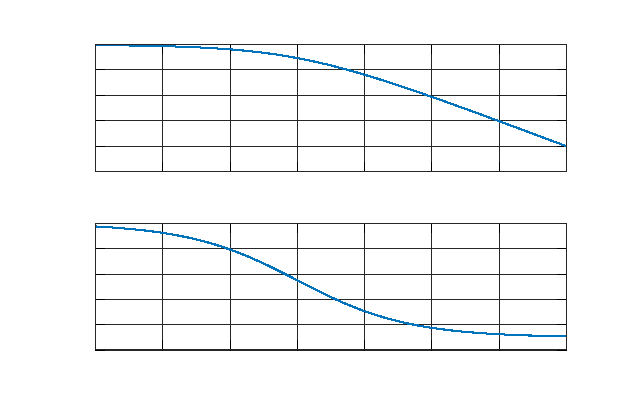
\includegraphics[width={291.60bp},height={180.00bp}]{fracfreqex1}}%
    \gplfronttext
  \end{picture}%
\endgroup
